\chapter{\label{ch1-intro}Introduction} 

\minitoc

\section{Cherenkov Radiation}

\begin{figure}
  \begin{subfigure}[b]{0.49\textwidth}
    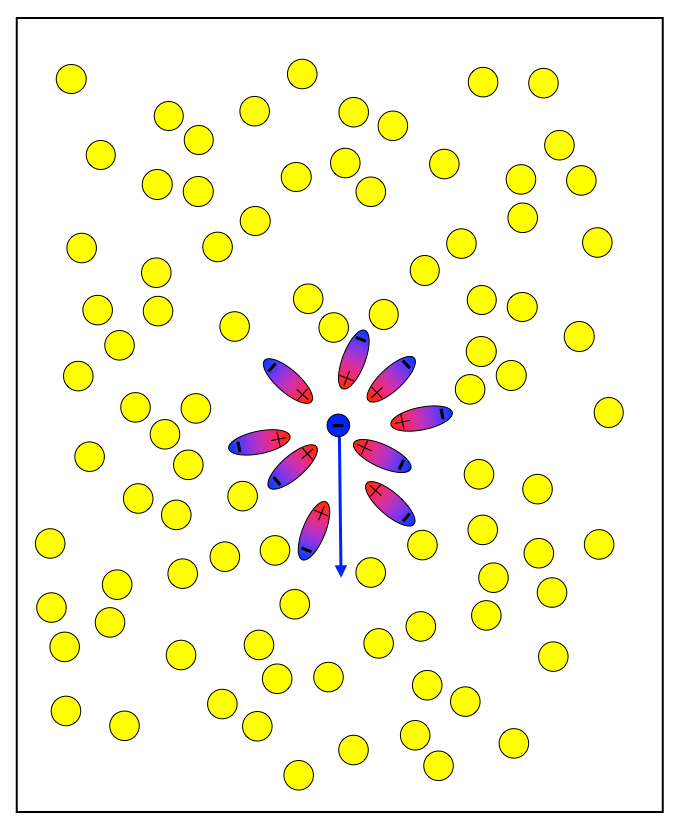
\includegraphics[width=\textwidth]{dipole_slow}
    \caption{$v < \frac{c}{n}$}
    \label{fig:dipole_slow}
  \end{subfigure}
  \hfill
  \begin{subfigure}[b]{0.49\textwidth}
    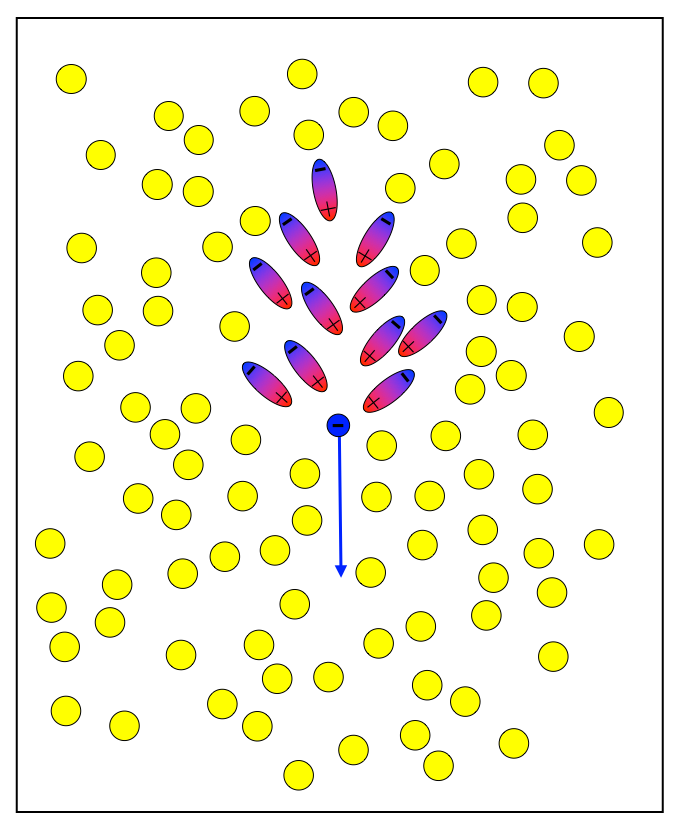
\includegraphics[width=\textwidth]{dipole_fast}
    \caption{$v \ge \frac{c}{n}$}
    \label{fig:dipole_fast}
  \end{subfigure}
  \caption[Polarisation produced in a dielectric medium due to the presence of a charged particle.]{Polarisation produced in a dielectric medium due to the presence of a charged particle, for the cases of a non-relativistic and relativistic particle.}
\end{figure}

\begin{figure}
	\centering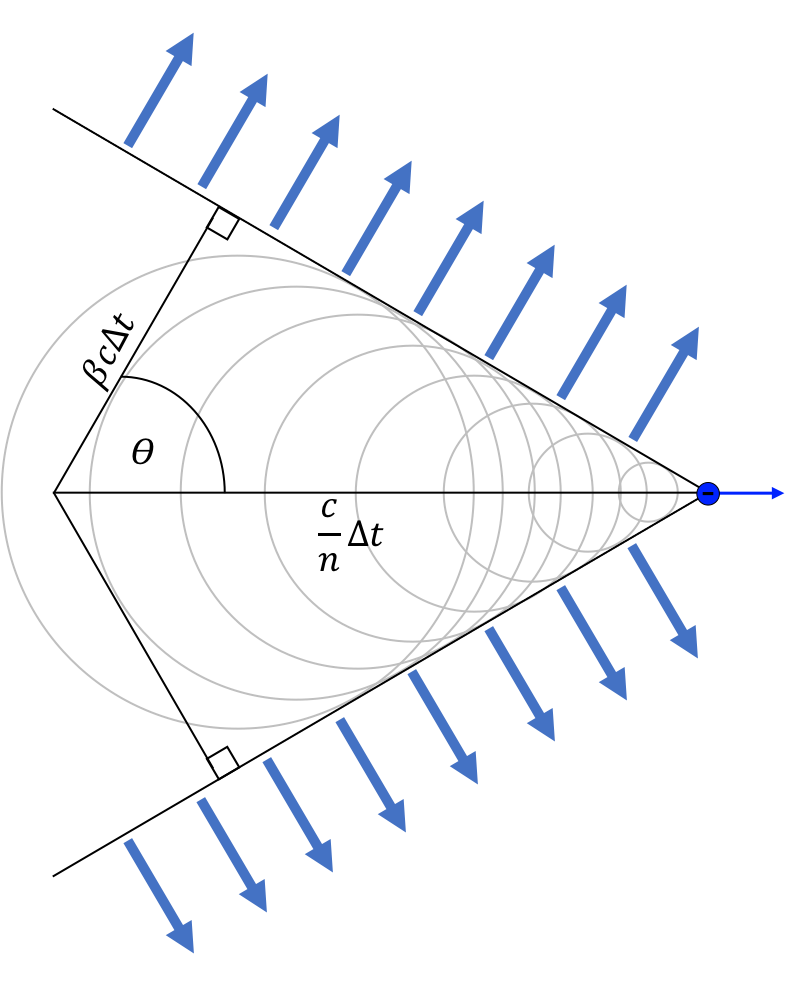
\includegraphics[width=0.5\textwidth]{cherenkov_geom} 
	\caption[Geometry of the wavefronts involved in Cherenkov radiation production.]{Geometry of the wavefronts involved in Cherenkov radiation production. The particle travels at a greater speed than the wavefronts propagate.}
	\label{fig:cherenkov_geom}
\end{figure}

When a charged particle moves slowly through a dielectric medium, the electric field of the particle distorts the nearby atoms. Momentarily, these atoms are transformed into elementary dipoles where the charged particles that constitute the atom are arranged with respect to the electric field of the travelling particle (Figure~\ref{fig:dipole_slow}). Due to the complete symmetry of this polarisation around the travelling particle, no net field is produced by the dielectric medium. However, if instead the velocity of the charged particle is faster than the speed light travels in that medium, an asymmetry along the particle trajectory is formed in the polarisation of the surrounding atoms (Figure~\ref{fig:dipole_fast}), resulting in a net dipole field. As the particle continues through the medium, elements of the polarised medium will release a brief burst of electromagnetic radiation. Generally these electromagnetic waves interfere destructively, except inside in the forward direction along the particles trajectory in an opening angle $\theta$. Although the full characterisation of this relativistic effect is complex, a simple consideration of the geometry involved, shown in Figure~\ref{fig:cherenkov_geom}, can be used to describe $\theta$ \cite{Jelley1958a}. In a time $\Delta t$ a particle travels a distance $\beta c \Delta t$ where $\beta = \frac{v}{c}$, while the emitted light will travel a distance $\frac{c}{n} \Delta t$ in a medium with refractive index $n$. This results in the relation:
\begin{equation} \label{eq:cherenkov_angle}
\cos \theta = \frac{c}{vn}.
\end{equation}
The blue light emitted in this constrained opening angle, via this phenomena, is known as Cherenkov radiation.

\section{Atmospheric Cherenkov Showers} \label{section:cherenkov_shower_intro}

\begin{figure}
	\centering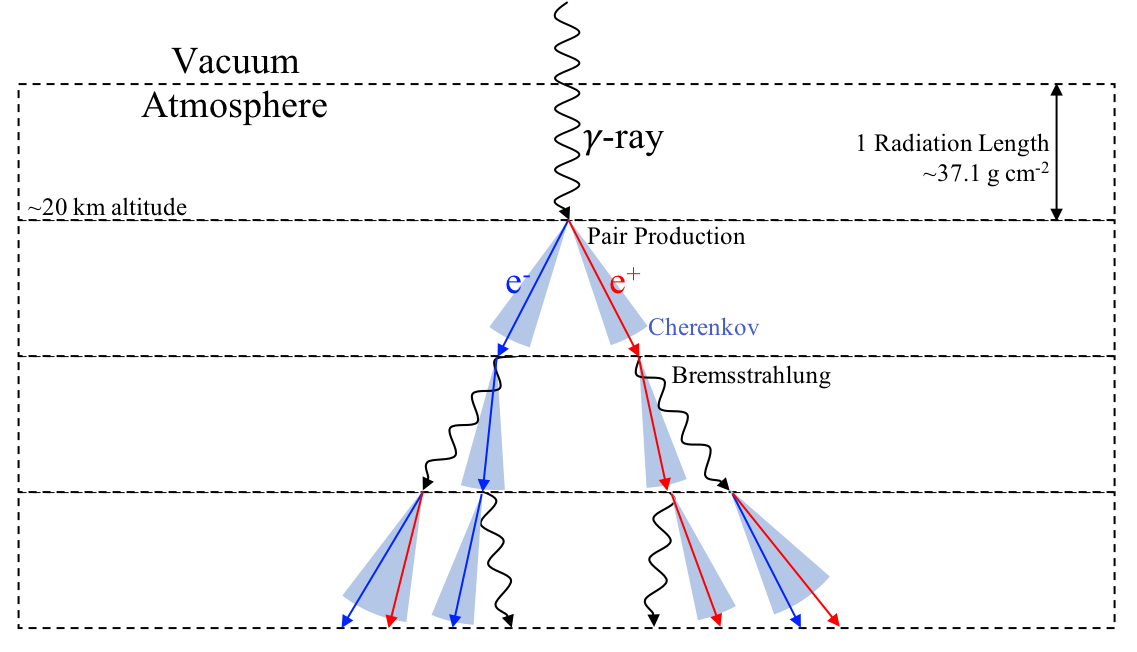
\includegraphics[width=\textwidth]{cascade} 
	\caption[Production of a extended electromagnetic particle cascade.]{Production of a extended electromagnetic particle cascade, demonstrating the different components and interactions.}
	\label{fig:cascade}
\end{figure}

The Earth's atmosphere is effectively opaque to photon energies above \SI{10}{eV} \cite{Weekes2003}. To perform astronomy at higher energies, one must usually leave the Earth's atmosphere. However, at energies above \SI{\ge 10}{GeV}, a ``gamma-ray window'' exists where astronomy can be performed using the Cherenkov radiation produced by the cascade of particles resulting from the interaction between the gamma ray and the atmosphere.

Two electromagnetic interactions are responsible for the creation of this cascade:
\begin{description}
\item [Pair Production] The conversion of a photon into an electron-positron pair in the presence of an atom (such as an atmospheric particle). The energy of the photon must exceed the sum of the rest masses of an electron and positron (\SI{1.022}{MeV}). The electron-positron pair share the energy of the progenitor photon, and continue on a similar trajectory. This is the dominating interaction process for photons above \SI{\ge 10}{MeV} \cite{Weekes2003}.
\item [Bremsstrahlung radiation] The emission of a photon due to the interaction of a charged particle with the electric field on an atom (such as an atmospheric particle). This process allows further gamma rays to be produced.
\end{description}
The interplay between these two processes, occurring after each transversal of a radiation length, produces the extensive cascade of energetic electromagnetic particles. This is illustrated in Figure~\ref{fig:cascade}. The charged particles produced by the pair production in this cascade are responsible for the generation of the Cherenkov light. This cascade is often known as a ``Cherenkov shower''.

This cascade continues until the ionisation energy losses are equal to the radiation losses. This number of remaining particles after this point, known as the ``shower maximum'' begins to diminish. For a \SI{1}{TeV} shower this occurs at \SI{\sim 8.4}{km} altitude \cite{Weekes2003}. The produced Cherenkov light is collimated along the progenitor gamma ray trajectory, and produces a pool of blue light on the ground, with a radius of \SI{\sim 120}{m} \cite{Hillas1996a}. If the direction of the Cherenkov shower is extrapolated back to the cosmic sphere, the location of the source that produced the gamma ray can be inferred. Although the amount of energy that goes into Cherenkov photon production is a tiny fraction of the total energy, the atmosphere acts as a consistent calorimeter, therefore allowing an accurate reconstruction of the progenitors energy from the amount of Cherenkov photons produced. 

A further characteristic of the Cherenkov shower is the time profile. The entire shower typically lasts \SI{\sim 5}{ns}. Therefore, despite the abundance of showers in the sky, and the visible wavelength of the Cherenkov light, they are imperceivable by the human eye. Furthermore, due to the faster-than-light velocities of the particles inside the cascade, the last Cherenkov photons produced at the end of the shower reach the ground before the first Cherenkov photons produced at the start of the shower. With different sections of the showers arriving at different times, the Cherenkov shower measurements display a time gradient across the image. 

\section{Imaging Atmospheric Cherenkov Telescopes}

A primary issue in \gls{vhe} astronomy is the low flux (${\sim} 0.2$ per \si{m \squared} per year \cite{Franco2016}), requiring a collection area that is not feasible for space telescopes. If instead the Cherenkov showers are used to detect the gamma rays, large arrays of optical telescopes can be built to provide stereoscopic imaging of the Cherenkov showers. These telescopes are known as \glspl{iact}. The multiple stereoscopic views of individual showers provided by arrays of \glspl{iact} allow accurate reconstruction of the properties of the shower, such as direction and energy. The topic of reconstruction is discussed in Chapter~\ref{ch6-reduction}.

As the \gls{iact} technique involves imaging the Cherenkov showers, which are much larger than typical astronomy targets, \glspl{iact} do not require the resolving power of typical optical telescopes. Instead the priorities of an \gls{iact} optical system are to maximise: 
\begin{itemize}
\item Mirror collection area, such that more photons can be collected. This enables fainter showers to be detected, thereby lowering the energy threshold.
\item \gls{fov}, which improves the surveying capabilities and eases the study of extended sources.
\end{itemize}
Furthermore, the large collection area provided by the light pool of the Cherenkov shower enables a modest telescope to still make a large amount of gamma ray detections, enabling this technique to be viable despite the small flux.

\begin{figure}
	\centering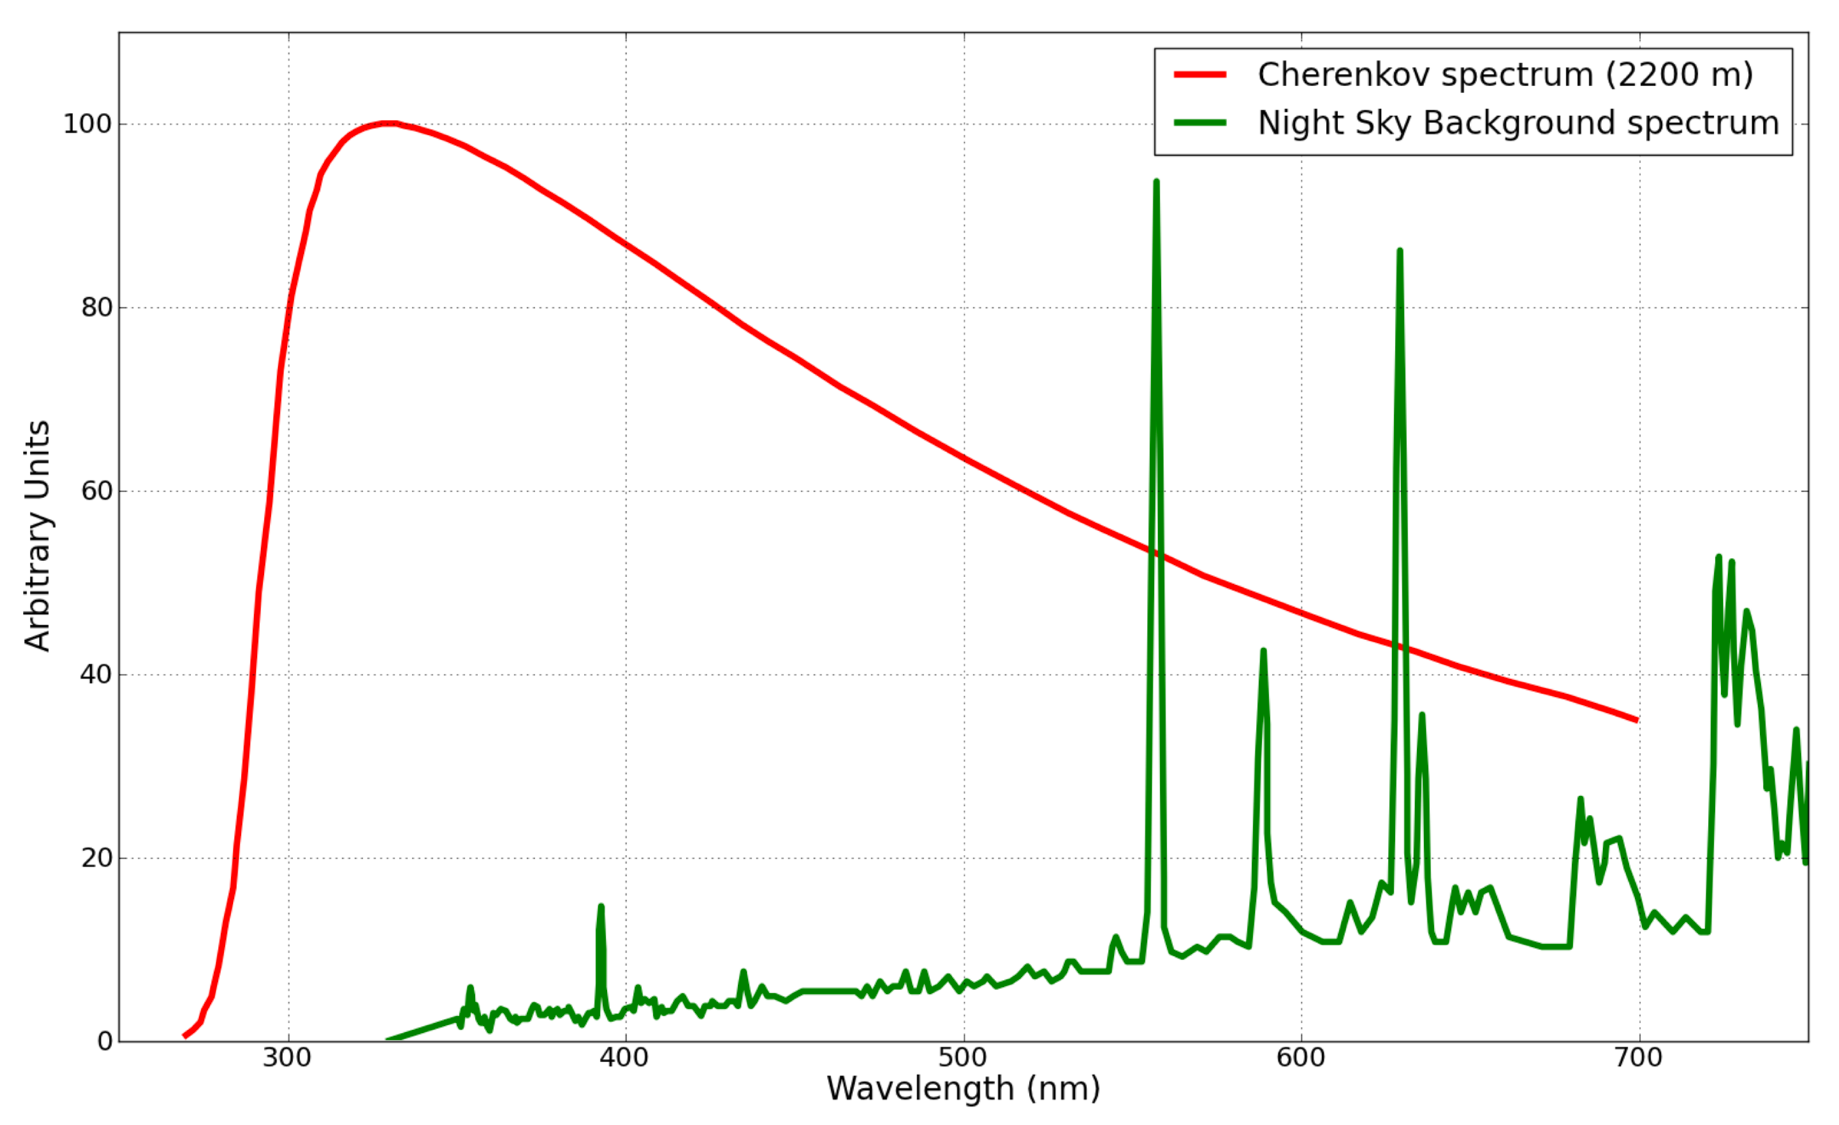
\includegraphics[width=\textwidth]{nsb} 
	\caption[Comparison of Cherenkov and NSB spectrum.]{Comparison of Cherenkov and NSB spectrum. The Cherenkov spectrum shown is expected at an altitude of \SI{2200}{m}. The NSB spectrum shown was measured at La Palma \cite{Bouvier2013}.}
	\label{fig:nsb}
\end{figure}

Two major background components need to be accounted for in \glspl{iact}:
\begin{description}
\item [Cosmic Ray Background] Protons (and heavier hadronic nuclei) are also capable of producing Cherenkov showers that are not entirely dissimilar to electromagnetic showers. As these particles are charged, they have been deflected by interstellar magnetic fields on their journey from their source, and therefore are not useful for \glspl{iact}. Therefore these showers provide an isotropic background which is 1,000 times as numerous than the shower rate received from the discreet gamma-ray sources. However, a hadronic shower exhibits a morphology that is broader and less symmetric than that obtained from gamma-ray showers. Additionally, distinct features such as ``muon rings'', produced by highly penetrating muons reaching low altitudes such that the full Cherenkov cone is visible in a single telescope, accompany hadronic showers. Parametrisations of the Cherenkov shower image therefore enable the discrimination of the hadronic showers (see Chapter~\ref{ch6-reduction}. \change{images?}
\item [Night Sky Background] Due to the optical sensitivity of the cameras used by \glspl{iact}, the measurements taken are susceptible to starlight, moonlight, and artificial light pollution. The \gls{nsb} spectrum for La Palma, compared to the expected Cherenkov spectrum at an altitude of \SI{2200}{m}, is displayed in Figure~\ref{fig:nsb}. This background is excluded in two ways. Firstly, smart trigger logic and strict thresholds (such as the one described in Chapter~\ref{ch2-mechanics}) eliminate the triggering on \gls{nsb} photons. Secondly, unbiased charge extraction technique (described in Chapter~\ref{ch6-reduction}) exclude this noise from the signal.
\end{description}

The application of the \gls{iact} technique was first attempted in the 1960s, but the first large optical reflector built with the purpose of gamma-ray astronomy was the Whipple 10 m telescope in southern Arizona, 1968. At first, gamma-ray astronomy was polluted with unsubstantial claims of transient signals from a variety of pulsars and binaries, but these signals had marginal statistical significance \cite[][p.~9]{Weekes2003}. It wasn't until 20 years later, after further development of the technique, that the Crab Nebula was detected by Whipple in 1989, thus reigniting interest in the development of gamma-ray astronomy.

\begin{figure}
  \centering
  \begin{subfigure}[b]{0.35\textwidth}
  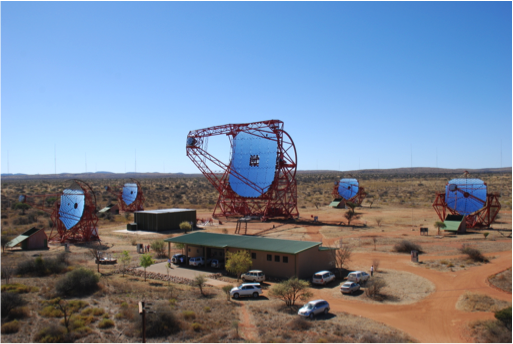
\includegraphics[width=\textwidth]{hess}
  \caption{H.E.S.S.}
  \label{fig:hess}
  \end{subfigure}
  ~
  \begin{subfigure}[b]{0.35\textwidth}
  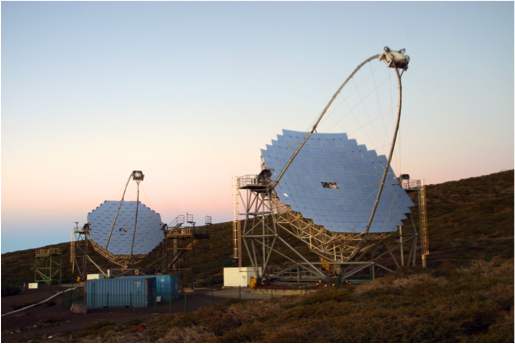
\includegraphics[width=\textwidth]{magic}
  \caption{MAGIC}
  \label{fig:magic}
  \end{subfigure}
  ~
  \begin{subfigure}[b]{0.45\textwidth}
  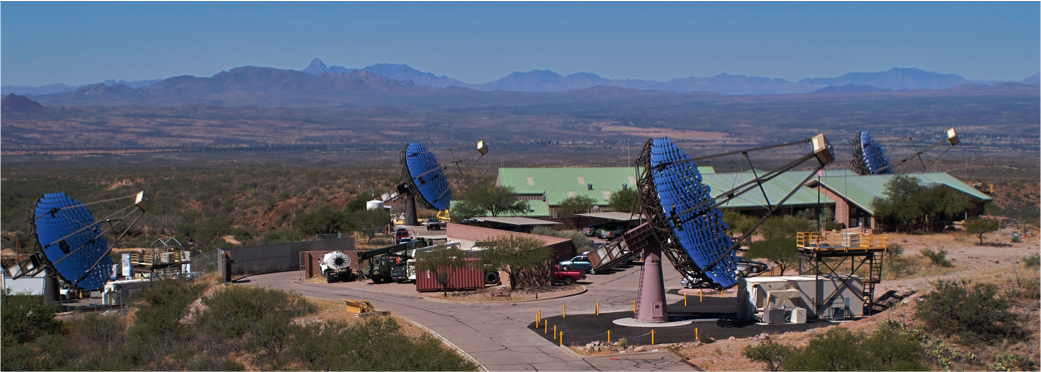
\includegraphics[width=\textwidth]{veritas}
  \caption{VERITAS}
  \label{fig:veritas}
  \end{subfigure}
  \caption{Photos of modern \glspl{iact}.}
  \label{fig:iacts}
\end{figure}

\begin{figure}
	\centering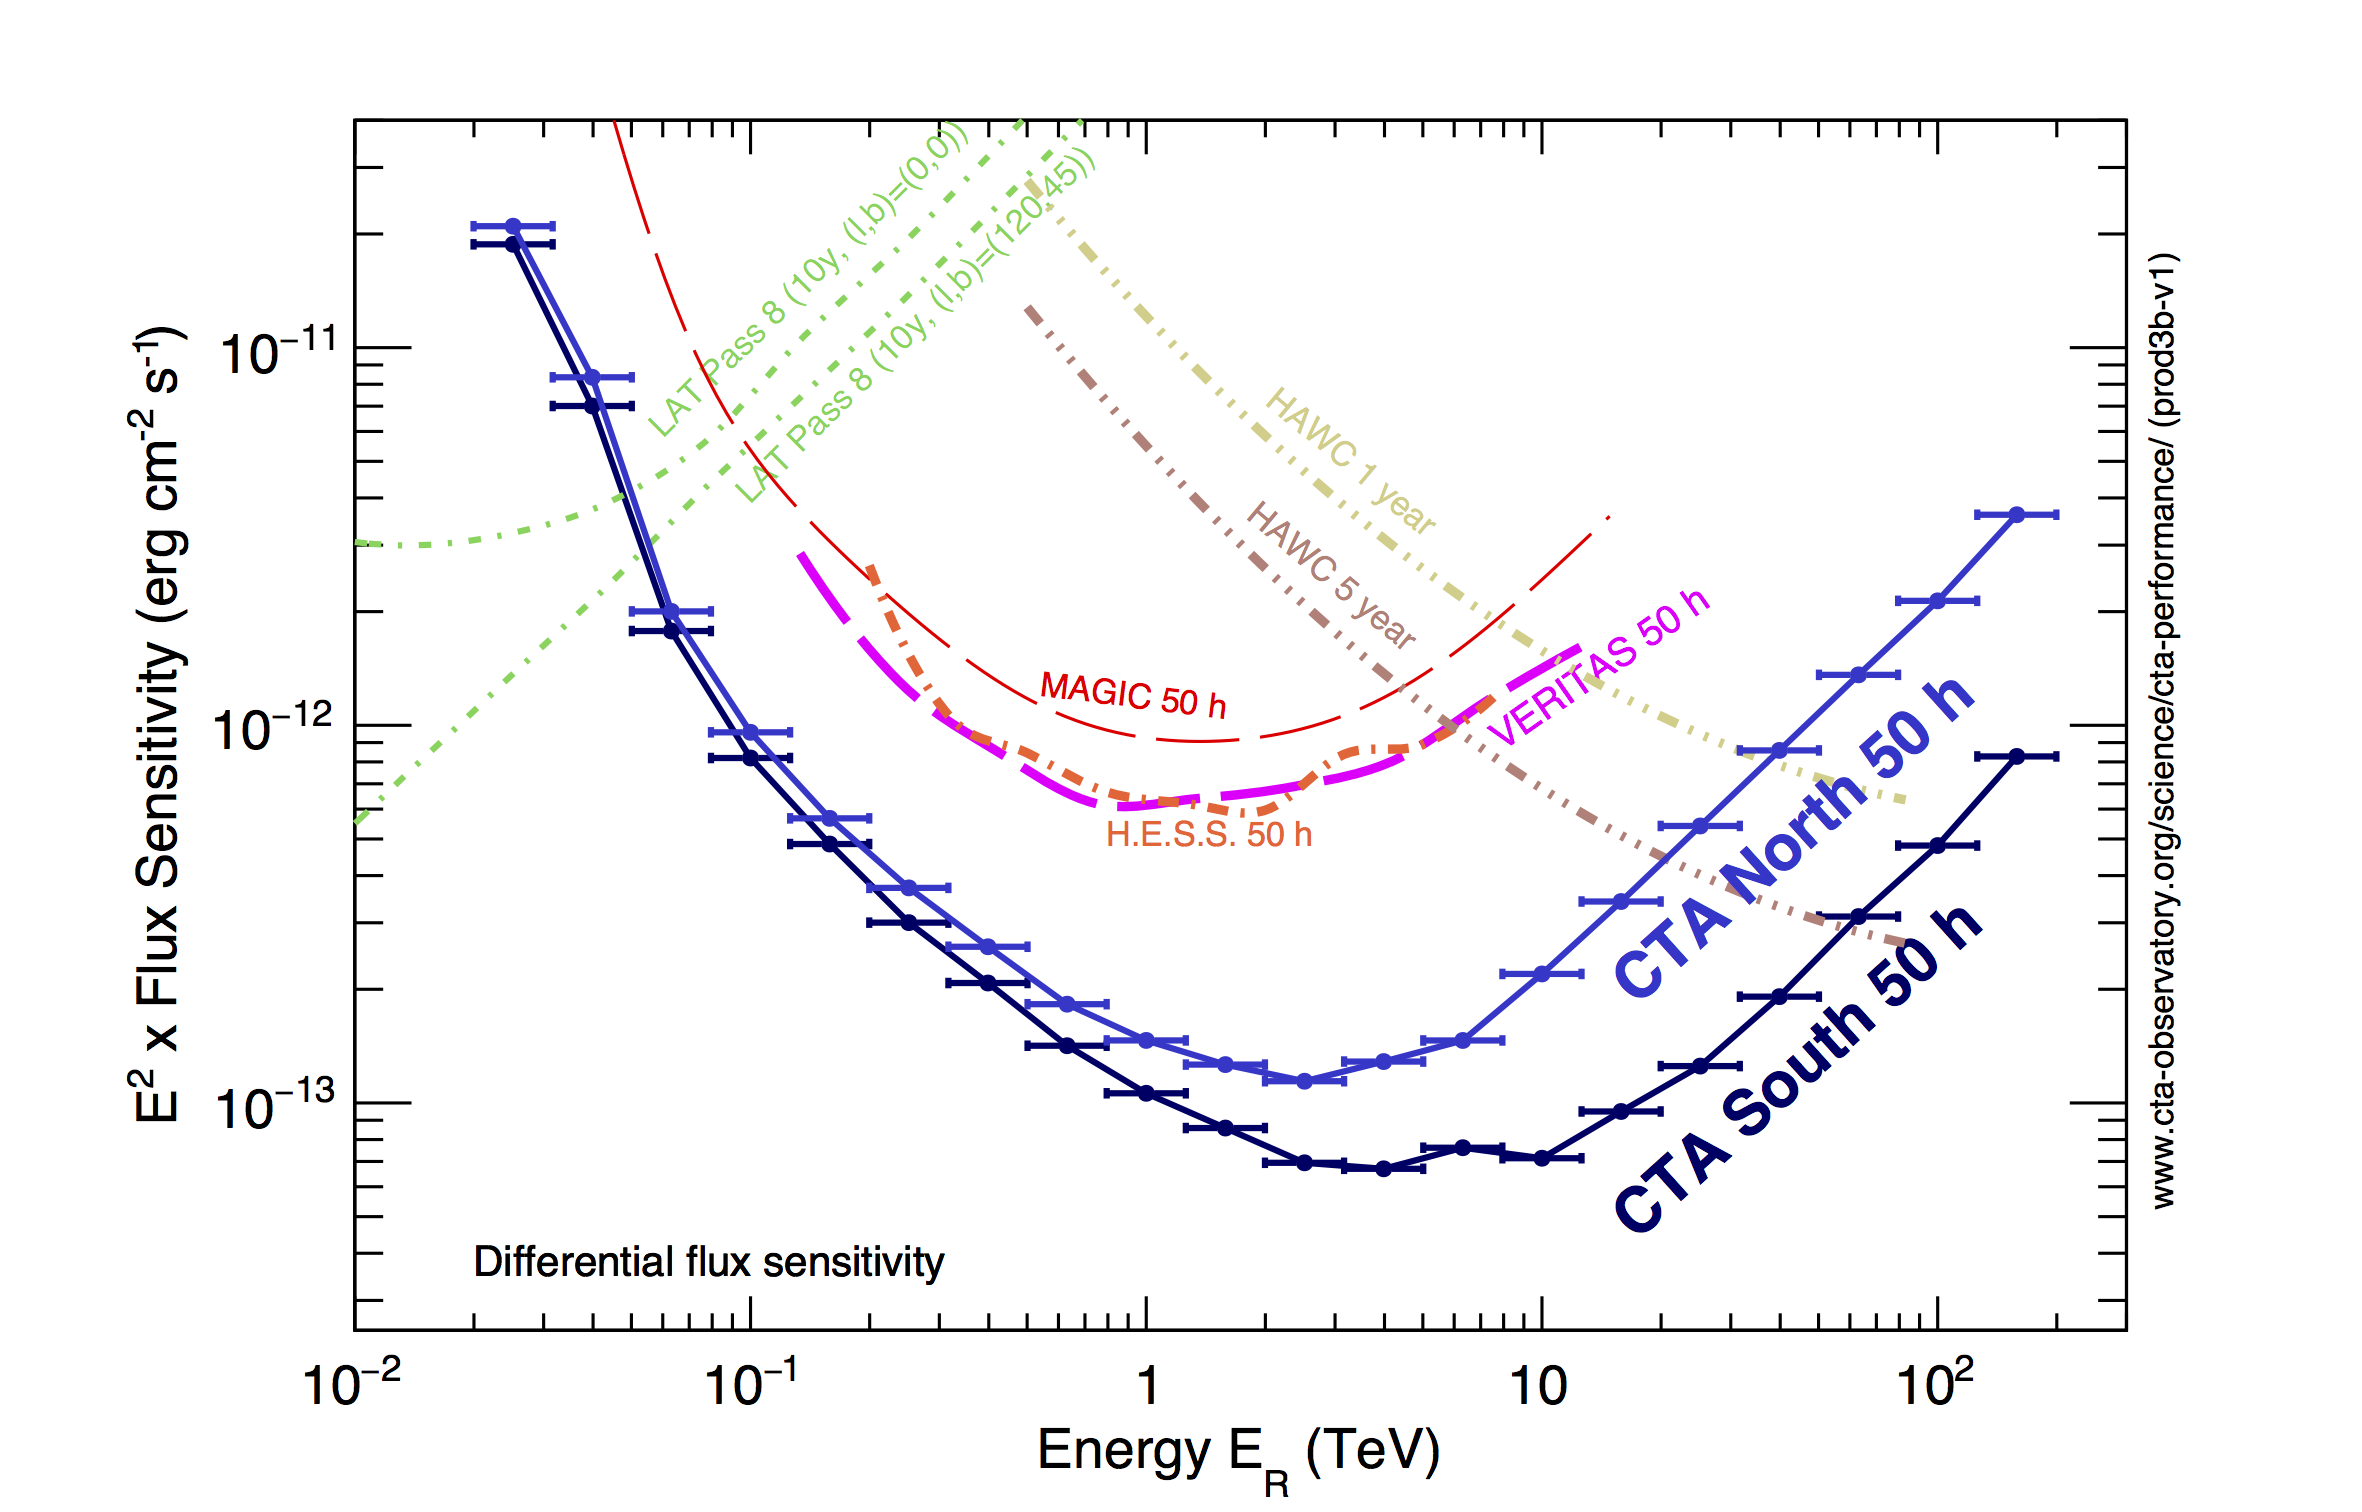
\includegraphics[width=\textwidth]{sensitivity} 
	\caption[Differential sensitivity of CTA.]{Differential sensitivity of CTA predicted by Monte Carlo simulations, compared to the performance of other gamma-ray instruments \cite{cta-performance}. The differential sensitivity has been defined as the minimum flux needed by CTA to obtain a 5-standard-deviation detection of a point-like source.}
	\label{fig:sensitivity}
\end{figure}

Modern \glspl{iact} include \gls{magic}, \gls{veritas}, and the most recent, \gls{hess} (Figure~\ref{fig:iacts}). All three of these telescope systems operate with the advantage of stereoscopic collaboration. In order to improve on the current \glspl{iact}, an array of ${\sim} 100$ telescopes was proposed, called the \gls{cta}. This array will have \cite{Acharya2013}:
\begin{itemize}
\item an improved sensitivity of 10 times over previous \glspl{iact} (Figure~\ref{fig:sensitivity}),
\item an observable gamma-ray energy range of \SI{30}{GeV} to \SI{100}{TeV},
\item a large (\SI{\sim 8}{\degree}) field of view for surveys,
\item improved angular and energy resolution,
\item and will be the first \gls{iact} to operate as an open observatory.
\end{itemize}

\section{The Cherenkov Telescope Array}

\begin{figure}
	\centering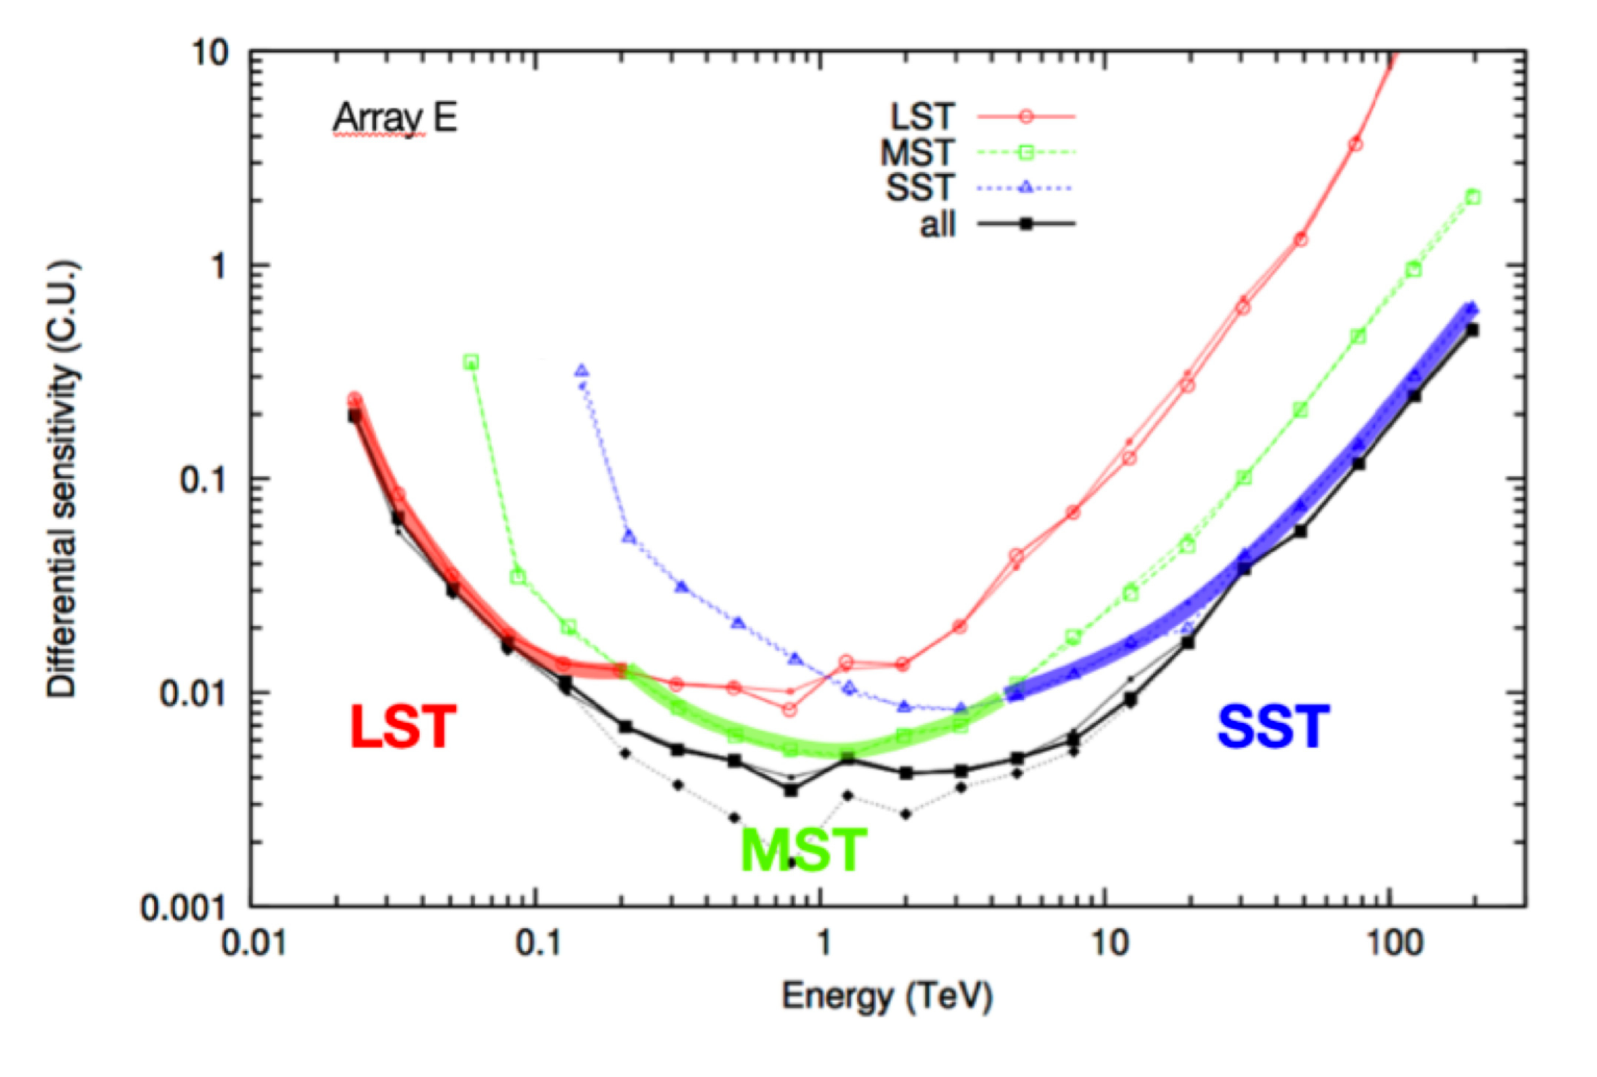
\includegraphics[width=\textwidth]{sensitivity_tel} 
	\caption[Differential sensitivity of the different CTA telescope types.]{Contribution of each telescope type within \gls{cta} to the total differential sensitivity \cite{Marano2014}.}
	\label{fig:sensitivity_tel}
\end{figure}

\gls{cta} will consist of three different sized telescopes:
\begin{itemize}
\item The \gls{lst}, with a mirror diameter of about \SI{23}{m} to enable the collection of as many photons as possible from the low energy showers (\SIrange{20}{150}{GeV}).
\item The \gls{mst}, covering the mid-range \SIrange{0.1}{10}{TeV} with mirror diameters of \SI{12}{m}.
\item The \gls{sst}, monitoring the high energies of \SIrange{1}{300}{TeV}, with mirror diameters of around \SI{4}{m}. Due to the rarity of higher energy showers, many \glspl{sst} need to be spread over an area of several square kilometres, to increase the chance of a detection \cite{Acharya2013}.
\end{itemize}
To illustrate these descriptions, the contributions of each telescope to the sensitivity of \gls{cta} is demonstrated in Figure~\ref{fig:sensitivity_tel}.

Two \gls{cta} sites will exist. A northern hemisphere site for extragalactic observations will be built at La Palma, and is planned to contain 4 \glspl{lst} and 16 \glspl{mst}. As this site will focus on the energy range from \SI{20}{GeV} to \SI{20}{TeV}, no \glspl{sst} are included on the northern site. A southern hemisphere site will provide observations of the galactic plane, spanning the full energy range of \gls{cta}. Planned to be built nearby the Paranal Observatory in the Atacama Desert in Chile, the southern array is planned to feature 4 \glspl{lst}, 15 \glspl{mst}, and 70 \glspl{sst}, spread over \SI{4}{km \squared}.

\section{Small Sized Telecopes}

Three designs for an \gls{sst} have been proposed:
\begin{itemize}
\item 
\end{itemize}


There exists 3 designs of the \gls{sst}: SST-1M (a single mirror design), ASTRI and \pgls{gct} (both being dual-mirror designs). These are shown in \autoref{fig:sst}. I am part of the \pgls{gct} group, which consists of the France-based GATE structure and mirrors, and the UK-based \gls{chec}. It is the development and commissioning of \gls{chec} that is the focus of my D.Phil. 

- Science with ssts
- Three designs

\section{Gamma-ray Cherenkov Telescope}

- what makes us better - lightweight telescope, full waveform readout
- optics








\notes[inline,caption={}]{
	\section{Plan}
	\subsection{Topics}
	\begin{itemize}
		\item High Energy Astrophysics
		\begin{itemize}
			\item Fermi
			\item Fermi Bubbles
			\item HAWC
		\end{itemize}
		\item IACTs
		\item CTA
		\item CTA Science
		\begin{itemize}
			\item Science Cases
			\item Use "Science with CTA" paper
		\end{itemize}
		\item SSTs
		\item SST Science
		\begin{itemize}
			\item What do we contribute?
			\item What can't be done without us?
		\end{itemize}
		\item GCT
		\item CHEC
		\begin{itemize}
			\item What makes us better?
			\item Advantages of Schwarzchild-Couder
			\begin{itemize}
				\item Increased FoV
				\item Size
				\item Cost
			\end{itemize}
			\item Advantages of full waveform readout
			\item Other Advantages?
			\begin{itemize}
				\item Trigger
				\item Energy/power/voltage Requirements
				\item Commonalities (SCT)
			\end{itemize}
		\end{itemize}
	\end{itemize}
	\subsection{Questions}
	\begin{itemize}
		\item ?
	\end{itemize}
}

\change[inline]{Shower properties, photons from bottom of shower are received before those at the top as the particle travels faster than light. Good figure in \cite{Cogan2006}}
\change[inline]{Gamma/Hadron/Lepton}

\change[inline]{Terminology note: charge not used in terms of columns, it refers to counts of photoelectrons, for which mV and ADC are a proxy of. Do a ctrl-f at end to check how charge is used}

\change[inline]{trigger efficiency???}

\change[inline]{introduce SC optics with reference to "modern iteration for utilisation in Cherenkov shower described by \cite{Vassiliev2007}" Giro2017}

low number of photons above 50 TeV, very low, frontier

\section{Atmospheric Cherenkov Showers}

\section{Imaging Atmospheric Cherenkov Technique}

\subsection{Cherenkov Shower Characteristics}

\subsection{Photon Arrival Time} \label{section:photon_arrival_time}

\change[inline]{Quoted from Holder2005: The longitudinal development of an air shower is reflected in the long axis of the elliptical image recorded in the camera. The photon arrival time profile along this axis is largely a result of geometrical path length differences, and hence the shower core distance. As the shower particles move faster than the speed of light in air, when the shower has a small core distance Cherenkov light emitted from lower in the atmosphere is received at the telescope first. At large core distances, this situation is reversed, as the Cherenkov light travel time from the shower to the telescope dominates. The effect of this is to produce a timing gradient along the long axis of the image, the size and sign of which depend upon the core distance. For gamma-ray showers from a point source at the centre of the field of view, the shower core distance is directly related to the angular distance in the camera of the image from the source position.
Figure}

\section{The Cherenkov Telescope Array}

CTA will be, for the first time in VHE gamma-ray astronomy, operated as an open observatory.

\section{Small Sized Telescopes}

\section{Science with the Small Sized Telescopes}

